\documentclass[pscyr,nonums]{hedlab}
\usepackage[russian]{babel}
\usepackage[utf8]{inputenc}
\usepackage{graphicx}
\usepackage{listings}
\usepackage{subcaption}

\graphicspath{{images//}}

\labnum{1}
\labname{Введение в разработку Android-приложений.}
\student{Голубев А.~В.}

\begin{document}
    \makeheader
    \lstset{language=java, basicstyle=\tiny}

    \noindent\emph{Цель работы:} 
    \begin{enumerate}
        \item познакомится с инструментами разработки Android-приложения
        \item разобрать структуру типичного Android-приложения
        \item научиться запускать приложение на эмуляторе
        \item научиться тестировать приложение с помощью Dalvik Debug Monitor Server (DDMS)
    \end{enumerate}

    \noindent 1. Работа с кнопкой
    \lstinputlisting{code/button.java}

    \pagebreak

    \noindent 2. Работа с анимацией
    \lstinputlisting{code/animation.java}

    \noindent 3. Работа с GPS
    \lstinputlisting{code/gps.java}

    \begin{figure}[!ht]
        \centering
        \begin{subfigure}[b]{0.45\textwidth}
            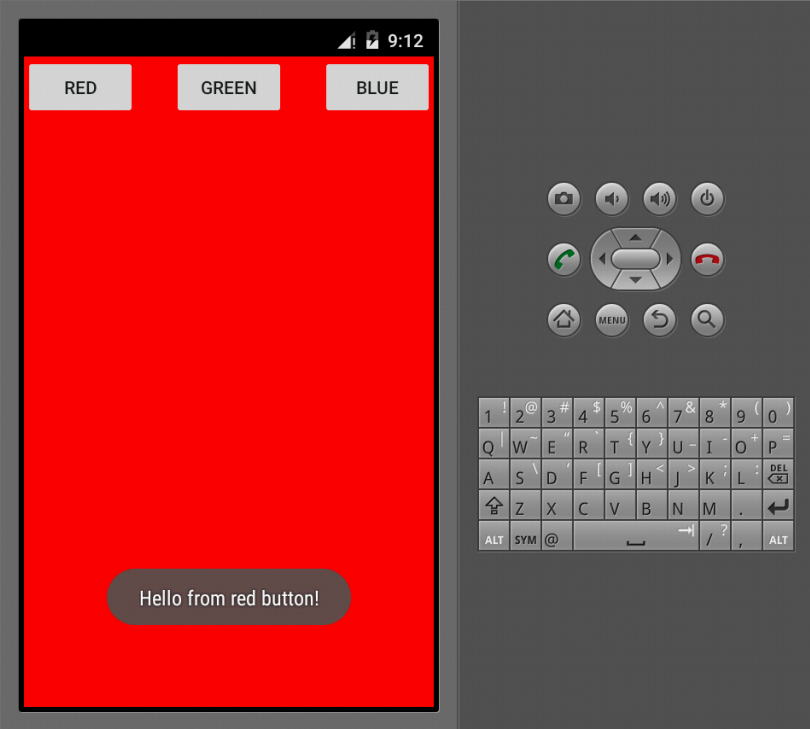
\includegraphics[width=\textwidth]{01}
            \caption{Screenshot приложения 1}
        \end{subfigure}
        \begin{subfigure}[b]{0.45\textwidth}
            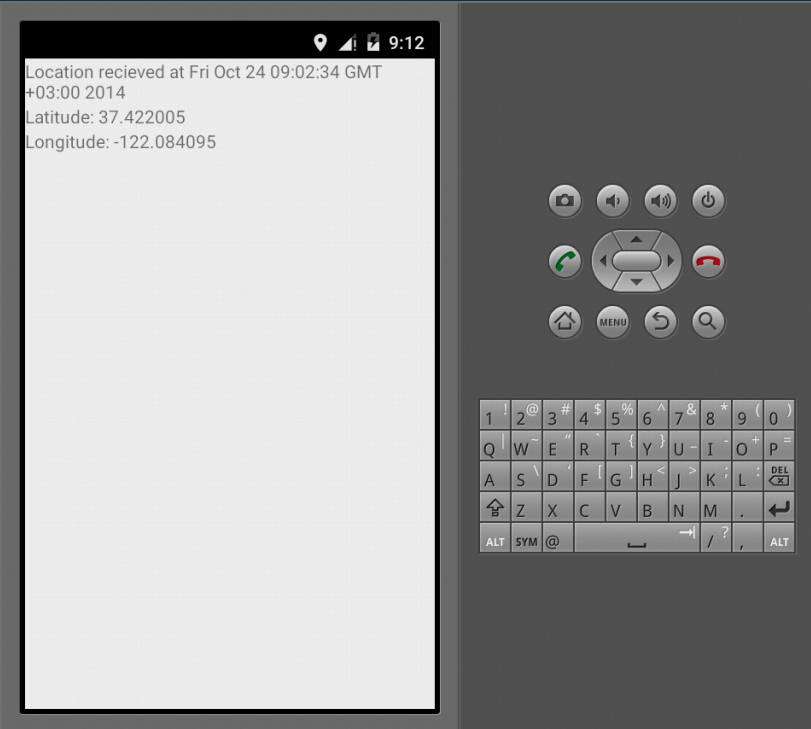
\includegraphics[width=\textwidth]{02}
            \caption{Screenshot приложения 1}
        \end{subfigure}
    \end{figure}
    \begin{figure}
        \center
        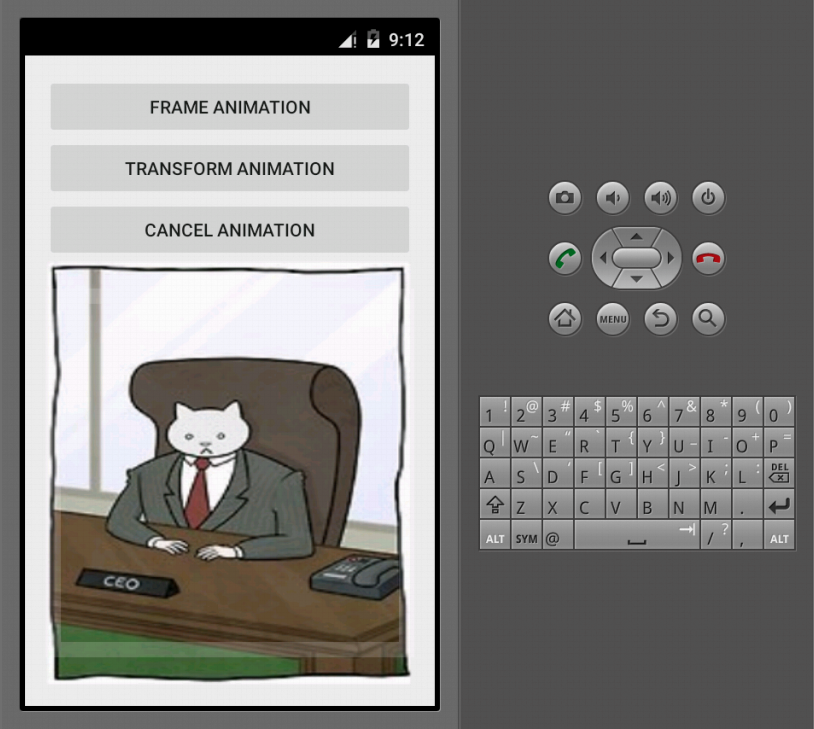
\includegraphics[width=0.45\textwidth]{03}
        \caption{Screenshot приложения 3}
    \end{figure}
\end{document}
